\documentclass{beamer}

\usepackage[utf8]{inputenc}
\usepackage[T1]{fontenc}
\usepackage{graphicx}
\usepackage{booktabs}
\usepackage{array}
\usepackage{amsmath}
\usepackage{amssymb}
\usepackage{colortbl}
\usepackage{tikz}
\usepackage{pgfgantt}
\usetikzlibrary{arrows.meta, positioning, fit}

\graphicspath{{figures_en/}}

% Graphviz figures: the dot code is written by filecontents* and compiled by dot.
% Needs shell escape (enabled by default on Overleaf, -shell-escape locally).
\usepackage{shellesc}
\newcommand{\compiledot}[1]{\ShellEscape{dot -Tpdf #1.dot -o #1.pdf}}
% Falls back on the exported PDF of figures_en/ when dot could not run
\newcommand{\dotfigure}[2]{%
  \IfFileExists{#1.pdf}
    {\includegraphics[width=\textwidth,height=0.9\textheight,keepaspectratio]{#1.pdf}}
    {\includegraphics[width=\textwidth,height=0.9\textheight,keepaspectratio]{#2}}}
% Diagram beside text, generated by dot; a reminder replaces it when shell escape is off
\newcommand{\dotdiagram}[1]{%
  \IfFileExists{#1.pdf}
    {\includegraphics[width=\linewidth,height=0.82\textheight,keepaspectratio]{#1.pdf}}
    {\fbox{\scriptsize Schéma Graphviz : compiler avec shell escape}}}
\ifnum\ShellEscapeStatus=1\else
  \PackageWarningNoLine{presentation}{Shell escape is off: the Graphviz figures use the PDFs of figures_en/}
\fi

\title{Analyse pharmaceutique assistée par IA}
\author{Isen Naiken}
\institute{CHU Dijon Bourgogne}
\date{\today}
\usetheme{Madrid}
\usecolortheme{default}
\setbeamertemplate{navigation symbols}{}

% Palette based on the blue of the application
\definecolor{puiblue}{RGB}{11,79,138}
\definecolor{puigreen}{RGB}{30,122,90}
% Colors of the Graphviz diagrams, reused in the TikZ diagrams
\definecolor{nodeblue}{HTML}{E9EEF4}
\definecolor{nodeline}{HTML}{3A3A3A}
\usecolortheme[named=puiblue]{structure}
\setbeamertemplate{blocks}[rounded][shadow=false]
\setbeamercolor{block title example}{bg=puigreen,fg=white}
\setbeamercolor{block body example}{bg=puigreen!8,fg=black}
\setbeamerfont{block title}{series=\bfseries}

% Code listings for the CLIPS, Python and JSON excerpts
\usepackage{listings}
\lstdefinelanguage{CLIPS}{
  morekeywords={defrule, deffacts, deftemplate, assert, not, declare, salience, slot, multislot},
  sensitive=true, morecomment=[l]{;}, morestring=[b]"}
\lstdefinelanguage{json}{morestring=[b]"}
\lstset{
  basicstyle=\ttfamily\scriptsize, columns=fullflexible, keepspaces=true,
  keywordstyle=\color{puiblue}\bfseries, commentstyle=\color{gray}\itshape,
  stringstyle=\color{puigreen}, showstringspaces=false,
  backgroundcolor=\color{puiblue!4}, frame=single, rulecolor=\color{puiblue!25},
  framesep=3pt, xleftmargin=3pt, xrightmargin=3pt, aboveskip=4pt, belowskip=4pt,
  literate={é}{{\'e}}1 {è}{{\`e}}1 {ê}{{\^e}}1 {à}{{\`a}}1 {ç}{{\c{c}}}1
           {É}{{\'E}}1 {µ}{{$\mu$}}1 {—}{{---}}1 {≥}{{$\geq$}}1 {ô}{{\^o}}1
}

% CLIPS keyword in a table cell
\newcommand{\clipskw}[1]{\textcolor{puiblue}{\textbf{#1}}}
% CLIPS fact in a table cell
\newcommand{\clipsfact}[1]{{\tiny\texttt{#1}}}

% Small heading in the theme color, used instead of a box
\newcommand{\heading}[1]{\par\medskip\structure{\textbf{#1}}\par\smallskip}

\begin{document}

\begin{frame}
  \titlepage
\end{frame}

\begin{frame}{Personnel et collaborateurs impliqués dans le projet}
  \centering
  \scriptsize
  \renewcommand{\arraystretch}{1.0}
  \setlength{\tabcolsep}{4pt}
  \begin{tabular}{>{\raggedright\arraybackslash}p{2.9cm}>{\raggedright\arraybackslash}p{3.0cm}>{\raggedright\arraybackslash}p{5.0cm}}
    \toprule
    \textbf{Nom \& Prénom} & \textbf{Fonction / Statut} & \textbf{Rattachements \& Équipes} \\
    \midrule
    AWAIS Muhammad & Stagiaire M2R ingénierie biomédicale & INSERM 1231 -- Équipe HSP-pathies \\
    BOULIN Mathieu & PUPH & PUI -- pôle pharmacie \\
    BRICQ Stéphanie & PU & ICube -- CNRS -- Strasbourg \\
    BRIOTTET Lucie & Stagiaire Ingénieur & École des Mines -- Saint-Étienne \newline Équipe D.I.A.D -- pôle biologie \\
    CALLEGARIN Davide & PH & Équipe D.I.A.D -- pôle biologie \\
    CALLIER Patrick & PUPH -- chef de service & Équipe D.I.A.D -- pôle biologie \\
    FOUQUIER Bastian & PH & PUI -- pôle pharmacie \\
    GOBBO Jessica & Chercheuse-clinicienne & UPP -- CGFL \newline INSERM 1231 -- Équipe HSP-pathies \\
    GUENFOUDI Marie-Pierre & PH -- cheffe de service & PUI -- pôle pharmacie \\
    NAIKEN Isen & Interne -- Doctorant Informatique & PUI -- pôle pharmacie \newline Équipe D.I.A.D -- pôle biologie \newline INSERM 1231 -- Équipe HSP-pathies \newline UBE -- ImVIA \\
    OPALE Mélodie & Ingénieur IA -- Data & Équipe D.I.A.D -- pôle biologie \\
    \bottomrule
  \end{tabular}

  \vspace{0.3em}
  \raggedright
  \tiny
  * D.I.A.D : Développement de l'Intelligence Artificielle \\
  * ImVIA : laboratoire Imagerie et Vision Artificielle
\end{frame}

\begin{frame}{Contexte}
  \heading{Objectif}
  Développer un modèle d'IA capable d'évaluer :
  \begin{itemize}
    \item le niveau de risque iatrogène ;
    \item la nécessité d'ajuster la prise en charge du patient.
  \end{itemize}
  \smallskip
  À partir des prescriptions et des données du Dossier Patient Informatisé (DPI).
  \vspace{0.6em}
  \begin{exampleblock}{Finalité}
    \centering Optimiser le ciblage des interventions pharmaceutiques (IP).
  \end{exampleblock}

  \heading{Liens du projet}
  \scriptsize
  \urlstyle{same}
  \renewcommand{\arraystretch}{1.1}
  \begin{tabular}{@{}ll@{}}
    \structure{\textbf{Code source (GitHub)}} & \url{https://github.com/naikenisen/projet_pui} \\
    \structure{\textbf{Démonstration (Streamlit)}} & \url{https://projetpui.streamlit.app/} \\
    \structure{\textbf{Manuscrit (Overleaf)}} & \url{https://www.overleaf.com/project/6afa1a238e5e3d2a0436ffc8} \\
  \end{tabular}
\end{frame}

\begin{frame}{Calendrier du projet}
  \centering
  \begin{ganttchart}[
      hgrid={*1{draw=black!10}}, vgrid={*1{draw=black!10}},
      x unit=1.08cm, y unit title=0.45cm, y unit chart=0.45cm,
      title/.style={fill=puiblue, draw=white},
      title label font=\scriptsize\bfseries\color{white},
      title height=1,
      group/.style={fill=puiblue, draw=none},
      group label font=\scriptsize\bfseries\color{puiblue},
      group height=.3, group top shift=.35, group peaks height=0, group peaks width=0, group left shift=0, group right shift=0,
      bar/.style={fill=puiblue!35, draw=none},
      bar label font=\tiny,
      bar height=.6, bar top shift=.2
    ]{1}{6}
    \gantttitle{2026}{2} \gantttitle{2027}{4} \\
    \gantttitle{nov.}{1} \gantttitle{déc.}{1} \gantttitle{janv.}{1}
    \gantttitle{févr.}{1} \gantttitle{mars}{1} \gantttitle{avr.}{1} \\
    \ganttgroup{Phase 1 : base de données}{1}{2} \\
    \ganttbar{Extraction SAP/BO, jointure des tables}{1}{2} \\
    \ganttbar{Anonymisation (métriques d'anonymat)}{2}{2} \\
    \ganttgroup{Phase 2 : architecture}{2}{3} \\
    \ganttbar{Revue de la littérature, méthodes SOTA}{2}{2} \\
    \ganttbar{Pipeline IA, briques sur mesure}{3}{3} \\
    \ganttgroup{Phase 3 : entraînement et prototype}{3}{5} \\
    \ganttbar{Entraînement, évaluation rétrospective}{4}{5} \\
    \ganttbar{Interface graphique (GUI), en parallèle}{3}{5} \\
    \ganttgroup{Phase 4 : valorisation}{5}{6} \\
    \ganttbar{Article rang A, puis open source}{5}{6} \\
    \ganttbar{Dialogue Stratégique, appels à projets}{6}{6}
  \end{ganttchart}
\end{frame}

\begin{frame}{Retombées attendues}
  \small
  \begin{itemize}
    \setlength{\itemsep}{0.6em}
    \item \structure{\textbf{Base de données réutilisable}} : riche, propre et structurée, directement utile à d'autres projets de recherche de la PUI.
    \item \structure{\textbf{Valorisation scientifique}} : publication des travaux et des résultats du modèle dans une revue internationale de rang A.
    \item \structure{\textbf{Partage méthodologique national}} : méthode et pipeline éprouvés, en libre accès, reproductibles par d'autres équipes hospitalières.
    \item \structure{\textbf{Intégration dans la pratique courante}} : déployer et tester l'outil en conditions réelles, pour aider les pharmaciens à cibler les interventions.
    \item \structure{\textbf{Cellule IA à la PUI}} : un pôle de compétences en IA au sein de la pharmacie, ouvert aux collaborations avec d'autres services cliniques et instituts de recherche.
  \end{itemize}
\end{frame}

\begin{filecontents*}[overwrite]{presentation_figure_1.dot}
// Figure 1 : architecture du pipeline
digraph architecture {
    graph [rankdir=LR, fontname="Helvetica", nodesep=0.45, ranksep=0.55, pad=0.15, newrank=true];
    node  [fontname="Helvetica", fontsize=10, color="#3A3A3A", penwidth=0.8];
    edge  [fontname="Helvetica", fontsize=8.5, color="#3A3A3A", arrowsize=0.7, penwidth=0.8];

    node [shape=folder, style=filled, fillcolor="#FFFFFF"];
    base     [label=<<B>RAG_Docs/</B><BR/><FONT POINT-SIZE="8.5">guidelines (PDF)</FONT>>];
    patients [shape=note, label=<<B>dataset/</B><BR/><FONT POINT-SIZE="8.5">one JSON file per patient</FONT>>];
    chroma   [shape=cylinder, label=<<B>chroma_db/</B><BR/><FONT POINT-SIZE="8.5">vector index</FONT>>];
    decision [shape=note, label=<<B>LLM decision</B><BR/><FONT POINT-SIZE="8.5">decision, points, sources</FONT>>];
    base_clp           [shape=note, label=<<B>base.clp</B><BR/><FONT POINT-SIZE="8.5">fact model, dose rules</FONT>>];
    generic_rules      [shape=note, label=<<B>generic_rules.clp</B><BR/><FONT POINT-SIZE="8.5">interactions (ANSM, DDI-Predictor)</FONT>>];
    personalized_rules [shape=note, label=<<B>personalized_rules.clp</B><BR/><FONT POINT-SIZE="8.5">hospital rules</FONT>>];

    node [shape=box, style="rounded,filled", fillcolor="#E9EEF4", margin="0.18,0.08"];
    indexing [label=<<B>indexing.py</B>>];
    main       [label=<<B>main.py</B><BR/><FONT POINT-SIZE="8.5">orchestration</FONT>>];
    retrieval      [label=<<B>retrieval.py</B><BR/><FONT POINT-SIZE="8.5">guideline passages</FONT>>];
    kbs        [label=<<B>kbs.py</B><BR/><FONT POINT-SIZE="8.5">KBS alerts</FONT>>];
    generation [label=<<B>generation.py</B>>];
    create_rule [label=<<B>create_rule.py</B><BR/><FONT POINT-SIZE="8.5">new KBS rules (LLM)</FONT>>];

    { rank=same; base; patients; create_rule; }
    { rank=same; indexing; main; base_clp; generic_rules; personalized_rules; }
    { rank=same; chroma; retrieval; kbs; }

    // Invisible edges keep the vertical order: RAG on top, rules at the bottom
    edge [style=invis];
    base -> patients -> create_rule;
    indexing -> main -> base_clp -> generic_rules -> personalized_rules;
    chroma -> retrieval -> kbs;
    edge [style=solid];

    base -> indexing -> chroma;
    chroma -> retrieval [style=dashed, label="read"];

    patients -> main;
    main -> generation;
    main -> retrieval;
    main -> kbs;
    retrieval -> generation;
    kbs -> generation;
    create_rule -> personalized_rules [label="new rule"];
    base_clp -> kbs [style=dashed];
    generic_rules -> kbs [style=dashed];
    personalized_rules -> kbs [style=dashed, label="read"];
    generation -> decision;
}
\end{filecontents*}
\compiledot{presentation_figure_1}

\begin{frame}
  \centering
  \dotfigure{presentation_figure_1}{figure_1.pdf}
\end{frame}

\begin{frame}{Principe de l'indexation (1/2)}
  \framesubtitle{Découpage du texte en passages, puis vectorisation}
  \centering
  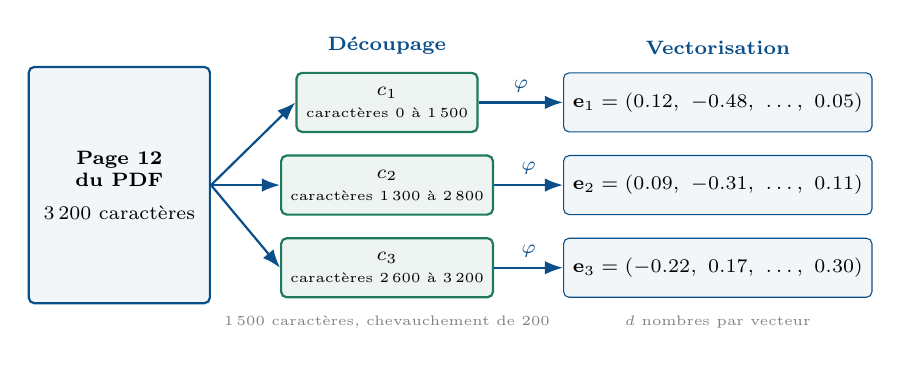
\begin{tikzpicture}[
      font=\scriptsize,
      box/.style={draw=puiblue, thick, rounded corners=2pt, align=center},
      passage/.style={draw=puigreen, thick, rounded corners=2pt, fill=puigreen!8, minimum width=2.3cm, minimum height=0.75cm, align=center},
      vector/.style={draw=puiblue, rounded corners=2pt, fill=puiblue!5, minimum width=3.9cm, minimum height=0.75cm},
      arrow/.style={-{Latex}, thick, puiblue}
    ]
    \node[box, fill=puiblue!5, minimum width=2.3cm, minimum height=3cm] (page) at (0,0)
      {\textbf{Page 12}\\ \textbf{du PDF}\\[4pt] 3\,200 caractères};
    \node[passage] (c1) at (3.4, 1.05) {$c_1$\\{\tiny caractères 0 à 1\,500}};
    \node[passage] (c2) at (3.4, 0)    {$c_2$\\{\tiny caractères 1\,300 à 2\,800}};
    \node[passage] (c3) at (3.4,-1.05) {$c_3$\\{\tiny caractères 2\,600 à 3\,200}};
    \node[vector] (e1) at (7.6, 1.05) {$\mathbf{e}_1 = (0.12,\ -0.48,\ \dots,\ 0.05)$};
    \node[vector] (e2) at (7.6, 0)    {$\mathbf{e}_2 = (0.09,\ -0.31,\ \dots,\ 0.11)$};
    \node[vector] (e3) at (7.6,-1.05) {$\mathbf{e}_3 = (-0.22,\ 0.17,\ \dots,\ 0.30)$};
    \foreach \k in {1,2,3} {
      \draw[arrow] (page.east) -- (c\k.west);
      \draw[arrow] (c\k.east) -- node[above] {$\varphi$} (e\k.west);
    }
    \node[above=0.1cm of c1, puiblue] {\textbf{Découpage}};
    \node[above=0.1cm of e1, puiblue] {\textbf{Vectorisation}};
    \node[below=0.1cm of c3, align=center, text=gray] {\tiny 1\,500 caractères, chevauchement de 200};
    \node[below=0.1cm of e3, align=center, text=gray] {\tiny $d$ nombres par vecteur};
  \end{tikzpicture}

  \small
  \begin{equation*}
    \mathbf{e}_k = \varphi(c_k) = (e_{k,1},\ e_{k,2},\ \dots,\ e_{k,d}) \in \mathbb{R}^{d}
  \end{equation*}
  \footnotesize
  \begin{tabular}{ll@{\qquad}ll}
    $c_k$ & texte du $k$-ième passage & $\varphi$ & modèle Qwen3-Embedding-8B \\
    $\mathbf{e}_k$ & vecteur du passage $c_k$ & $d$ & nombre de dimensions ($d = 4\,096$) \\
  \end{tabular}
\end{frame}

\begin{frame}{Principe de l'indexation (2/2)}
  \framesubtitle{La base vectorielle : une ligne par passage}
  \centering
  \footnotesize
  \renewcommand{\arraystretch}{1.4}
  \begin{tabular}{>{\raggedright\arraybackslash}p{4.5cm}ll}
    \toprule
    \textbf{Passage $c_k$} & \textbf{Vecteur $\mathbf{e}_k \in \mathbb{R}^d$} & \textbf{Page et lignes} \\
    \midrule
    $c_1$ : « Sujet âgé : apixaban 2,5 mg $\times$ 2/jour si\dots » & $(0.12,\ -0.48,\ \dots,\ 0.05)$ & p.~12, l.~1--25 \\
    $c_2$ : « \dots rivaroxaban contre-indiqué si ClCr $<$ 15\dots » & $(0.09,\ -0.31,\ \dots,\ 0.11)$ & p.~12, l.~22--48 \\
    $c_3$ : « \dots surveiller la fonction rénale chaque année\dots » & $(-0.22,\ 0.17,\ \dots,\ 0.30)$ & p.~12, l.~45--60 \\
    \multicolumn{1}{c}{$\vdots$} & \multicolumn{1}{c}{$\vdots$} & \multicolumn{1}{c}{$\vdots$} \\
    $c_N$ : « Daptomycine : 10 mg/kg/jour\dots » & $(-0.31,\ 0.07,\ \dots,\ 0.22)$ & p.~4, l.~8--30 \\
    \bottomrule
  \end{tabular}

  \vspace{1em}
  \begin{exampleblock}{Base vectorielle}
    \centering
    Tous les référentiels PDF $\rightarrow$ $N$ passages $\rightarrow$ $N$ lignes. \\
    Construite une seule fois, avant toute analyse de patient.
  \end{exampleblock}
\end{frame}

\begin{frame}{Principe de la récupération (1/2)}
  \framesubtitle{Vectorisation de la requête et similarité cosinus}
  \centering
  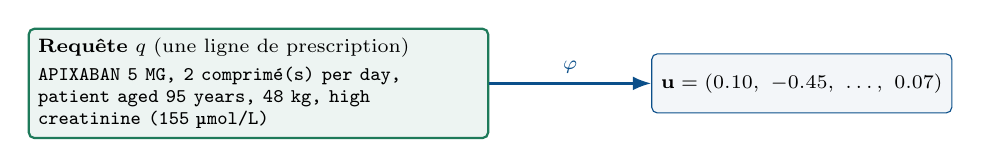
\begin{tikzpicture}[
      font=\scriptsize,
      arrow/.style={-{Latex}, thick, puiblue}
    ]
    \node[draw=puigreen, thick, rounded corners=2pt, fill=puigreen!8, text width=5.6cm, align=left] (q) at (0,0)
      {\textbf{Requête $q$} (une ligne de prescription)\\[2pt]
       \texttt{\scriptsize APIXABAN 5 MG, 2 comprimé(s) per day, patient aged 95 years, 48 kg, high creatinine (155 µmol/L)}};
    \node[draw=puiblue, rounded corners=2pt, fill=puiblue!5, minimum height=0.75cm] (u) at (6.9,0)
      {$\mathbf{u} = (0.10,\ -0.45,\ \dots,\ 0.07)$};
    \draw[arrow] (q.east) -- node[above] {$\varphi$} (u.west);
  \end{tikzpicture}

  \raggedright
  \small
  La requête est vectorisée avec le même modèle, dans le même espace que les passages :
  \begin{equation*}
    \mathbf{u} = \varphi(q) = (u_1,\ u_2,\ \dots,\ u_d) \in \mathbb{R}^{d}
  \end{equation*}
  On compare $\mathbf{u}$ au vecteur $\mathbf{e}_k$ de chaque ligne de la base :
  \begin{equation*}
    \cos(\mathbf{u}, \mathbf{e}_k) = \frac{\mathbf{u} \cdot \mathbf{e}_k}{\|\mathbf{u}\|\,\|\mathbf{e}_k\|}
    = \frac{\sum_{i=1}^{d} u_i\, e_{k,i}}{\sqrt{\sum_{i=1}^{d} u_i^2}\ \sqrt{\sum_{i=1}^{d} e_{k,i}^2}}
  \end{equation*}
  {\footnotesize Proche de 1 : même sens. Proche de 0 : textes sans rapport. On garde la ligne la plus proche :}
  \[ k^* = \operatorname*{arg\,max}_{k \in \{1, \dots, N\}} \cos(\mathbf{u}, \mathbf{e}_k) \]
\end{frame}

\begin{frame}{Principe de la récupération (2/2)}
  \framesubtitle{Recherche de la ligne la plus proche dans la base}
  \centering
  \scriptsize
  \renewcommand{\arraystretch}{1.4}
  \begin{tabular}{>{\raggedright\arraybackslash}p{3.9cm}ll|c}
    \toprule
    \textbf{Passage $c_k$} & \textbf{Vecteur $\mathbf{e}_k \in \mathbb{R}^d$} & \textbf{Page et lignes} & $\boldsymbol{\cos(\mathbf{u}, \mathbf{e}_k)}$ \\
    \midrule
    \rowcolor{puigreen!15}
    $c_1$ : « Sujet âgé : apixaban 2,5 mg $\times$ 2/jour si\dots » & $(0.12,\ -0.48,\ \dots,\ 0.05)$ & p.~12, l.~1--25 & \textbf{0.91} \\
    $c_2$ : « \dots rivaroxaban contre-indiqué si ClCr $<$ 15\dots » & $(0.09,\ -0.31,\ \dots,\ 0.11)$ & p.~12, l.~22--48 & 0.64 \\
    $c_3$ : « \dots surveiller la fonction rénale chaque année\dots » & $(-0.22,\ 0.17,\ \dots,\ 0.30)$ & p.~12, l.~45--60 & 0.38 \\
    \multicolumn{1}{c}{$\vdots$} & \multicolumn{1}{c}{$\vdots$} & \multicolumn{1}{c|}{$\vdots$} & $\vdots$ \\
    $c_N$ : « Daptomycine : 10 mg/kg/jour\dots » & $(-0.31,\ 0.07,\ \dots,\ 0.22)$ & p.~4, l.~8--30 & 0.12 \\
    \bottomrule
  \end{tabular}

  \vspace{0.6em}
  \small
  \begin{exampleblock}{Sortie : $k^* = 1$}
    \centering
    Le passage $c_1$ et sa provenance (p.~12, l.~1--25) sont envoyés au LLM.
  \end{exampleblock}
  {\scriptsize En pratique : les 3 passages les plus proches de chaque ligne de prescription, 8 au total par patient.}
\end{frame}

\begin{filecontents*}[overwrite]{presentation_figure_2a.dot}
// Figure 2a : RAG, clinical profile of the patient
digraph retrieval_profile {
    graph [rankdir=TB, fontname="Helvetica", fontsize=12, nodesep=0.25, ranksep=0.3, pad=0.05, newrank=true];
    node  [fontname="Helvetica", fontsize=12, color="#3A3A3A", penwidth=0.8,
           shape=box, style="rounded,filled", fillcolor="#E9EEF4", margin="0.1,0.05"];
    edge  [fontname="Helvetica", fontsize=10, color="#3A3A3A", arrowsize=0.7, penwidth=0.8];

    record [shape=note, style=filled, fillcolor="#FFFFFF", label=<<B>Patient record</B><BR/>age, weight<BR/>lab values<BR/>prescription lines>];
    ranges [shape=note, style=filled, fillcolor="#FFFFFF", label=<<B>Reference</B><BR/><B>ranges</B><BR/>[min, max]>];
    { rank=same; record; ranges; }

    bio [label=<<B>1. Abnormal lab values</B><BR/>&lt; min  →  “low …”<BR/>&gt; max  →  “high …”>];
    profile [shape=box, style=filled, fillcolor="#FFFFFF", label=<<B>Clinical profile T</B><BR/>age, weight,<BR/>abnormalities>];

    record -> bio;
    ranges -> bio;
    bio -> profile;
    record -> profile;
}
\end{filecontents*}
\compiledot{presentation_figure_2a}

\begin{frame}{Récupération des passages (RAG) (1/3)}
  \framesubtitle{Profil clinique du patient}
  \begin{columns}[c]
    \begin{column}{0.58\textwidth}
      \centering
      \dotdiagram{presentation_figure_2a}
    \end{column}
    \begin{column}{0.40\textwidth}
      \footnotesize
      \begin{itemize}
        \setlength{\itemsep}{0.6em}
        \item Le dossier donne l'âge, le poids, la biologie et les lignes de prescription.
        \item Chaque valeur biologique est comparée à son intervalle $[\min, \max]$.
        \item Hors de l'intervalle : anomalie, par exemple créatinine 155 $\mu$mol/L $\rightarrow$ « high creatinine ».
        \item Âge, poids et anomalies forment le profil $T$, commun à toutes les lignes.
      \end{itemize}
    \end{column}
  \end{columns}
\end{frame}

\begin{filecontents*}[overwrite]{presentation_figure_2b.dot}
// Figure 2b : RAG, one query per prescription line
digraph retrieval_query {
    graph [rankdir=TB, fontname="Helvetica", fontsize=12, nodesep=0.25, ranksep=0.3, pad=0.05, newrank=true];
    node  [fontname="Helvetica", fontsize=12, color="#3A3A3A", penwidth=0.8,
           shape=box, style="rounded,filled", fillcolor="#E9EEF4", margin="0.1,0.05"];
    edge  [fontname="Helvetica", fontsize=10, color="#3A3A3A", arrowsize=0.7, penwidth=0.8];

    profile [shape=box, style=filled, fillcolor="#FFFFFF", label=<<B>Profile T</B>>];
    line [shape=note, style=filled, fillcolor="#FFFFFF", label=<<B>Line L<SUB>i</SUB></B>>];
    { rank=same; profile; line; }

    subgraph cluster_iteration {
        label=<<B>2. For each line L<SUB>i</SUB></B>>;
        labelloc=b; labeljust=l; fontsize=12; style="dashed,rounded"; color="#6A6A6A"; margin=10;

        query [label=<<B>Query q<SUB>i</SUB></B><BR/>INN, dose,<BR/>regimen + T>];
        embed [label=<<B>Vector encoding</B><BR/>φ(instruction + q<SUB>i</SUB>)<BR/>→  u<SUB>i</SUB> ∈ ℝ<SUP>d</SUP>>];
        query -> embed;
    }

    profile -> query;
    line -> query;
}
\end{filecontents*}
\compiledot{presentation_figure_2b}

\begin{frame}{Récupération des passages (RAG) (2/3)}
  \framesubtitle{Une requête par ligne de prescription}
  \begin{columns}[c]
    \begin{column}{0.58\textwidth}
      \centering
      \dotdiagram{presentation_figure_2b}
    \end{column}
    \begin{column}{0.40\textwidth}
      \footnotesize
      \begin{itemize}
        \setlength{\itemsep}{0.6em}
        \item Chaque ligne $L_i$ donne une requête $q_i$ : médicament, dose, posologie, puis le profil $T$.
        \item \textit{Exemple :} « apixaban 5 mg, 1 tablet morning and evening, patient aged 95 years, 48 kg, high creatinine ».
        \item Précédée d'une instruction, la requête est vectorisée par Qwen3-Embedding-8B : $\mathbf{u}_i = \varphi(q_i)$.
        \item Les $n$ requêtes sont encodées en un seul appel.
      \end{itemize}
    \end{column}
  \end{columns}
\end{frame}

\begin{filecontents*}[overwrite]{presentation_figure_2c.dot}
// Figure 2c : RAG, nearest-neighbour search and merging
digraph retrieval_search {
    graph [rankdir=TB, fontname="Helvetica", fontsize=12, nodesep=0.25, ranksep=0.3, pad=0.05, newrank=true];
    node  [fontname="Helvetica", fontsize=12, color="#3A3A3A", penwidth=0.8,
           shape=box, style="rounded,filled", fillcolor="#E9EEF4", margin="0.1,0.05"];
    edge  [fontname="Helvetica", fontsize=10, color="#3A3A3A", arrowsize=0.7, penwidth=0.8];

    vectors [shape=note, style=filled, fillcolor="#FFFFFF", label=<<B>u<SUB>1</SUB>, …, u<SUB>n</SUB></B>>];
    chroma [shape=cylinder, style=filled, fillcolor="#FFFFFF", label=<<B>ChromaDB</B><BR/>index>];
    { rank=same; vectors; chroma; }

    knn [label=<<B>k-NN search</B><BR/>cosine, k = 3<BR/>per query>];
    fusion [label=<<B>3. Result merging</B><BR/>≤ 3n passages<BR/>duplicates: min d<BR/>top 8 selected>];
    output [shape=note, style=filled, fillcolor="#FFFFFF", label=<<B>Documentary context</B><BR/>≤ 8 excerpts<BR/>[source, page] text>];

    vectors -> knn;
    chroma -> knn [style=dashed];
    knn -> fusion;
    fusion -> output;
}
\end{filecontents*}
\compiledot{presentation_figure_2c}

\begin{frame}{Récupération des passages (RAG) (3/3)}
  \framesubtitle{Recherche dans la base et fusion des résultats}
  \begin{columns}[c]
    \begin{column}{0.58\textwidth}
      \centering
      \dotdiagram{presentation_figure_2c}
    \end{column}
    \begin{column}{0.40\textwidth}
      \footnotesize
      \begin{itemize}
        \setlength{\itemsep}{0.6em}
        \item Pour chaque $\mathbf{u}_i$ : les 3 passages les plus proches de la base (similarité cosinus).
        \item Au plus $3n$ passages ; un passage trouvé plusieurs fois garde sa plus petite distance.
        \item Tri par distance croissante, les 8 premiers sont gardés.
        \item Sortie : au plus 8 extraits « [source, page] texte », envoyés au LLM.
      \end{itemize}
    \end{column}
  \end{columns}
\end{frame}

\begin{filecontents*}[overwrite]{presentation_figure_3a.dot}
// Figure 3a : KBS, the three steps from the patient JSON to the alerts
digraph kbs_steps {
    graph [rankdir=TB, fontname="Helvetica", fontsize=12, nodesep=0.25, ranksep=0.3, pad=0.05, newrank=true];
    node  [fontname="Helvetica", fontsize=12, color="#3A3A3A", penwidth=0.8,
           shape=box, style="rounded,filled", fillcolor="#E9EEF4", margin="0.1,0.05"];
    edge  [fontname="Helvetica", fontsize=10, color="#3A3A3A", arrowsize=0.7, penwidth=0.8];

    record [shape=note, style=filled, fillcolor="#FFFFFF", label=<<B>Patient JSON</B>>];
    rules [shape=note, style=filled, fillcolor="#FFFFFF", label=<<B>.clp files</B><BR/><FONT POINT-SIZE="10.5">templates + rules</FONT>>];
    { rank=same; record; rules; }

    facts [label=<<B>1. assert_patient()</B><BR/>JSON  →  facts>];
    memory [fillcolor="#FFFFFF", label=<<B>Working memory</B>>];
    run [label=<<B>2. env.run()</B><BR/>rules fire, new facts>];
    read [label=<<B>3. apply_rules()</B><BR/>reads the alert facts>];
    output [shape=note, style=filled, fillcolor="#FFFFFF", label=<<B>Alert list</B><BR/>text  →  LLM>];

    record -> facts;
    facts -> memory [label=<  assert>];
    rules -> memory [label=<  load>];
    memory -> run;
    run -> memory [style=dashed, label=<  new facts>];
    run -> read;
    read -> output;
}
\end{filecontents*}
\compiledot{presentation_figure_3a}

\begin{frame}{Système à base de connaissances (KBS)}
  \framesubtitle{Du dossier JSON aux alertes, en trois étapes}
  \begin{columns}[c]
    \begin{column}{0.52\textwidth}
      \centering
      \dotdiagram{presentation_figure_3a}
    \end{column}
    \begin{column}{0.46\textwidth}
      \small
      \begin{enumerate}
        \setlength{\itemsep}{0.8em}
        \item \structure{\textbf{Faits}} : \texttt{kbs.py} traduit le JSON en faits CLIPS.
        \item \structure{\textbf{Inférence}} : CLIPS applique les règles des fichiers \texttt{.clp}.
        \item \structure{\textbf{Sortie}} : \texttt{kbs.py} relit les faits \texttt{alert}.
      \end{enumerate}
      \bigskip
      \footnotesize\textit{Exemple suivi : daptomycine 0,7 g par jour, patient de 80 kg.}
    \end{column}
  \end{columns}
\end{frame}

\begin{frame}[fragile]{Étape 1 : du JSON aux faits}
  \heading{Un fait = un modèle (\texttt{deftemplate}) + des champs (\texttt{slot})}
\begin{lstlisting}[language=CLIPS]
(deftemplate treatment (slot line) (slot quantity) (slot unit) ...)
\end{lstlisting}
  \heading{\texttt{kbs.py} crée les faits à partir du JSON}
  \centering
  \scriptsize
  \renewcommand{\arraystretch}{1.5}
  \begin{tabular}{>{\ttfamily\raggedright\arraybackslash}p{4cm} c >{\ttfamily\raggedright\arraybackslash}p{5.2cm}}
    \toprule
    \normalfont\textbf{JSON} & & \normalfont\textbf{Fait CLIPS} \\
    \midrule
    "weight\_kg": 80 & $\rightarrow$ & (data (name "weight\_kg") (value 80)) \\
    "quantity\_per\_day": 0.7 \newline "intake\_unit": "gramme(s)" & $\rightarrow$ & (treatment (line 0) (quantity 0.7) \newline \ \ (unit "gramme(s)")) \\
    "drug\_label": \newline "DAPTOMYCINE 350 MG\dots" & $\rightarrow$ & (prescribed (line 0) (drug "daptomycine")) \\
    \bottomrule
  \end{tabular}

  \medskip
  \raggedright
  \scriptsize
  \texttt{line 0} : première ligne de prescription. Le libellé donne un fait \texttt{prescribed} par suite de mots (« daptomycine », « 350 mg »\dots) : une règle reconnaît le médicament par simple égalité.
\end{frame}

\begin{frame}{Lire une règle CLIPS}
  \framesubtitle{La règle de la daptomycine, ligne par ligne}
  \centering
  \footnotesize
  \renewcommand{\arraystretch}{1.4}
  \begin{tabular}{>{\ttfamily}l>{\raggedright\arraybackslash}p{4.1cm}}
    \toprule
    \normalfont\textbf{Code CLIPS} & \textbf{Signification} \\
    \midrule
    (\clipskw{defrule} daptomycine-dose & une règle, et son nom \\
    \ \ (prescribed (line ?l) (drug \textcolor{puigreen}{"daptomycine"})) & \textbf{SI} la ligne \texttt{?l} contient « daptomycine » \\
    \ \ (dose-per-kg (line ?l) (mg ?mg\&:(< ?mg 10))) & \textbf{ET} sa dose par kg \texttt{?mg} est $<$ 10 \\
    \ \ \clipskw{=>} & \textbf{ALORS} \\
    \ \ (\clipskw{assert} (alert (message \textcolor{puigreen}{"\dots"}) (lines ?l)))) & ajouter un fait \texttt{alert} pour la ligne \texttt{?l} \\
    \bottomrule
  \end{tabular}

  \vspace{0.6em}
  \raggedright
  \footnotesize
  \begin{itemize}
    \setlength{\itemsep}{0.2em}
    \item \texttt{?l}, \texttt{?mg} : \structure{\textbf{variables}}, remplies avec les valeurs des faits trouvés.
    \item Le même \texttt{?l} dans les deux conditions : les deux faits doivent concerner la même ligne.
    \item \texttt{\&:( \dots )} ajoute un test sur la valeur.
  \end{itemize}
\end{frame}

\begin{frame}[fragile]{Les règles de calcul de \texttt{base.clp}}
  \framesubtitle{Le JSON ne contient pas de dose par kg : deux règles la calculent}
  \begin{columns}[T]
    \begin{column}{0.62\textwidth}
\begin{lstlisting}[language=CLIPS]
(deffacts units
  (unit-to-mg (unit "gramme(s)") (factor 1000))
  ...)

(defrule daily-dose-from-intake-unit
  (treatment (line ?l) (quantity ?q) (unit ?u))
  (unit-to-mg (unit ?u) (factor ?f))
  =>
  (assert (daily-dose (line ?l) (mg (* ?q ?f)))))

(defrule dose-per-kg
  (daily-dose (line ?l) (mg ?mg))
  (data (name "weight_kg") (value ?w))
  =>
  (assert (dose-per-kg (line ?l) (mg (/ ?mg ?w)))))
\end{lstlisting}
    \end{column}
    \begin{column}{0.36\textwidth}
      \small
      \vspace{0.3em}
      \structure{\textbf{Faits fixes}} \\
      {\footnotesize 1 g = 1\,000 mg}

      \vspace{2.2em}
      \structure{\textbf{Dose par jour}} \\
      {\footnotesize 0,7 $\times$ 1\,000 = 700 mg}

      \vspace{3.2em}
      \structure{\textbf{Dose par kg}} \\
      {\footnotesize 700 / 80 = 8,75 mg/kg}
    \end{column}
  \end{columns}
  \scriptsize
  \textit{Conditions simplifiées : le fichier vérifie aussi que la quantité et le poids sont positifs.}
\end{frame}

\begin{frame}{Étape 2 : le chaînage des règles}
  \framesubtitle{Chaque fait ajouté déclenche la règle suivante}
  \centering
  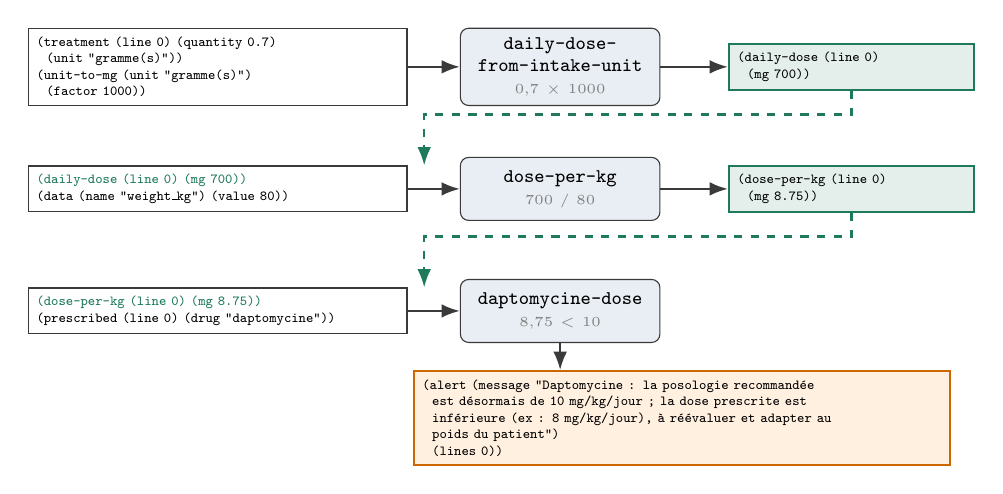
\begin{tikzpicture}[
      font=\tiny,
      facts/.style={draw=nodeline, fill=white, align=left, font=\tiny\ttfamily, text width=4.6cm, inner sep=3pt},
      rule/.style={draw=nodeline, rounded corners=3pt, fill=nodeblue, align=center, font=\scriptsize\ttfamily, minimum height=0.8cm, text width=2.3cm},
      new/.style={draw=puigreen, thick, fill=puigreen!12, align=left, font=\tiny\ttfamily, text width=2.9cm, inner sep=3pt},
      arrow/.style={-{Latex}, thick, nodeline}
    ]
    \node[facts] (in1) at (0, 0) {(treatment (line 0) (quantity 0.7)\\\ \ (unit "gramme(s)"))\\(unit-to-mg (unit "gramme(s)")\\\ \ (factor 1000))};
    \node[rule] (r1) at (4.35, 0) {daily-dose-\\from-intake-unit\\{\tiny\rmfamily\color{gray} 0,7 $\times$ 1000}};
    \node[new] (out1) at (8.05, 0) {(daily-dose (line 0)\\\ \ (mg 700))};

    \node[facts] (in2) at (0, -1.55) {\textcolor{puigreen}{\textbf{(daily-dose (line 0) (mg 700))}}\\(data (name "weight\_kg") (value 80))};
    \node[rule] (r2) at (4.35, -1.55) {dose-per-kg\\{\tiny\rmfamily\color{gray} 700 / 80}};
    \node[new] (out2) at (8.05, -1.55) {(dose-per-kg (line 0)\\\ \ (mg 8.75))};

    \node[facts] (in3) at (0, -3.1) {\textcolor{puigreen}{\textbf{(dose-per-kg (line 0) (mg 8.75))}}\\(prescribed (line 0) (drug "daptomycine"))};
    \node[rule] (r3) at (4.35, -3.1) {daptomycine-dose\\{\tiny\rmfamily\color{gray} 8,75 $<$ 10}};
    \node[new, draw=orange!80!black, fill=orange!12, text width=6.6cm, anchor=north] (out3) at (5.9, -3.85)
      {(alert (message "Daptomycine : la posologie recommandée\\\ \ est désormais de 10 mg/kg/jour ; la dose prescrite est\\\ \ inférieure (ex : 8 mg/kg/jour), à réévaluer et adapter au\\\ \ poids du patient")\\\ \ (lines 0))};

    \foreach \k in {1,2} {
      \draw[arrow] (in\k) -- (r\k);
      \draw[arrow] (r\k) -- (out\k);
    }
    \draw[arrow] (in3) -- (r3);
    \draw[arrow] (r3.south) -- (r3.south |- out3.north);
    \draw[arrow, dashed, puigreen] (out1.south) -- ++(0, -0.3) -| ([xshift=6pt]in2.north east);
    \draw[arrow, dashed, puigreen] (out2.south) -- ++(0, -0.3) -| ([xshift=6pt]in3.north east);
  \end{tikzpicture}

  \vspace{0.3em}
  \footnotesize
  Ensuite, plus aucune règle ne s'applique : l'inférence s'arrête avec 1 alerte.
\end{frame}

\begin{filecontents*}[overwrite]{presentation_figure_4.dot}
// Figure 4 : génération de l'avis pharmaceutique par le LLM (generation.py)
digraph generation {
    graph [rankdir=TB, fontname="Helvetica", fontsize=10, nodesep=0.35, ranksep=0.4, pad=0.15, newrank=true];
    node  [fontname="Helvetica", fontsize=9.5, color="#3A3A3A", penwidth=0.8,
           shape=box, style="rounded,filled", fillcolor="#E9EEF4", margin="0.16,0.08"];
    edge  [fontname="Helvetica", fontsize=8.5, color="#3A3A3A", arrowsize=0.7, penwidth=0.8];

    node [shape=note, style=filled, fillcolor="#FFFFFF"];
    record  [label=<<B>Patient record</B><BR/>JSON: patient + treatments>];
    alerts  [label=<<B>Alerts A</B><BR/><FONT POINT-SIZE="8.5">KBS (Figure 3)</FONT>>];
    context [label=<<B>Documentary context</B><BR/><FONT POINT-SIZE="8.5">retrieval (Figure 2)</FONT>>];
    { rank=same; record; alerts; context; }

    node [shape=box, style="rounded,filled", fillcolor="#E9EEF4"];

    prompt [shape=note, style=filled, fillcolor="#FFFFFF", label=<<TABLE BORDER="0" CELLSPACING="0" CELLPADDING="1">
        <TR><TD ALIGN="LEFT"><B>System prompt</B></TD></TR>
        <TR><TD ALIGN="LEFT">role: French hospital clinical pharmacist</TD></TR>
        <TR><TD ALIGN="LEFT">no diagnosis in the record: each point relies on a fact,</TD></TR>
        <TR><TD ALIGN="LEFT">an alert or an excerpt</TD></TR>
        <TR><TD ALIGN="LEFT">ANSM alert levels (CI, ASDEC, PE, APEC):</TD></TR>
        <TR><TD ALIGN="LEFT">an alert never justifies an intervention on its own</TD></TR>
        <TR><TD ALIGN="LEFT">consistency checks with laboratory values and dates</TD></TR>
        <TR><TD ALIGN="LEFT">4 point types · JSON response format</TD></TR>
        </TABLE>>];

    llm [label=<<B>1. Language model inference</B><BR/>Qwen3.6-35B-A3B (via OpenRouter)<BR/><FONT POINT-SIZE="8.5">temperature 0 · reasoning enabled · ≤ 12,000 tokens · JSON output</FONT>>];
    { rank=same; llm; prompt; }

    post [label=<<B>2. Post-processing</B><BR/>JSON parsing · [A] / [R] identifiers → alerts and documents<BR/>[L] identifiers → lines to modify (interventions only)<BR/>decision = most severe point>];

    output [shape=plain, label=<<TABLE BORDER="1" CELLBORDER="0" CELLSPACING="0" CELLPADDING="4" COLOR="#3A3A3A" BGCOLOR="#FFFFFF">
        <TR><TD COLSPAN="2" ALIGN="LEFT" BGCOLOR="#F2F2F2"><B>Pharmaceutical opinion</B></TD></TR>
        <TR><TD ALIGN="LEFT"><I>decision</I></TD><TD ALIGN="LEFT">PHARMACEUTICAL INTERVENTION  &gt;  VERIFICATION  &gt;<BR ALIGN="LEFT"/>MONITORING PROPOSED  &gt;  PATIENT VALIDATED<BR ALIGN="LEFT"/></TD></TR>
        <TR><TD ALIGN="LEFT"><I>reasoning</I></TD><TD ALIGN="LEFT">3 to 6 sentences</TD></TR>
        <TR><TD ALIGN="LEFT"><I>points</I></TD><TD ALIGN="LEFT">1 to 4, each with a type, a short proposal (≤ 40 words),<BR ALIGN="LEFT"/>its sources and the lines to modify<BR ALIGN="LEFT"/></TD></TR>
        <TR><TD ALIGN="LEFT"><I>sources</I></TD><TD ALIGN="LEFT">KBS alerts and “file.pdf, page p”,<BR ALIGN="LEFT"/>or empty (model knowledge only)<BR ALIGN="LEFT"/></TD></TR>
        </TABLE>>];

    record -> llm;
    alerts -> llm [label=" user role"];
    context -> llm;
    prompt -> llm [label="system role"];
    llm -> post;
    post -> output;
}
\end{filecontents*}
\compiledot{presentation_figure_4}

\begin{frame}
  \centering
  \dotfigure{presentation_figure_4}{figure_4.pdf}
\end{frame}
\begin{frame}{MoE}
  \framesubtitle{\textit{Mixture of Experts} : chaque token n'utilise qu'une petite partie du modèle}
  \centering
  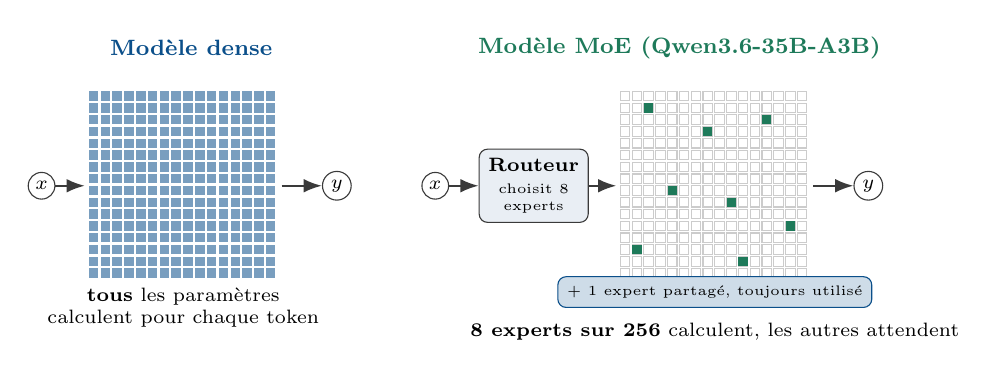
\begin{tikzpicture}[
      font=\scriptsize,
      token/.style={draw=nodeline, circle, fill=white, inner sep=1.5pt},
      box/.style={draw=nodeline, rounded corners=3pt, fill=nodeblue, align=center},
      arrow/.style={-{Latex}, thick, nodeline}
    ]
    % Dense model: every block computes
    \node[font=\footnotesize\bfseries, text=puiblue] at (1.9, 1.75) {Modèle dense};
    \node[token] (xd) at (0, 0) {$x$};
    \begin{scope}[shift={(0.6, 1.2)}]
      \foreach \i in {0,...,15} {
        \foreach \j in {0,...,15} {
          \fill[puiblue!55] (\i*0.15, -\j*0.15) rectangle ++(0.12, -0.12);
        }
      }
    \end{scope}
    \node[token] (yd) at (3.75, 0) {$y$};
    \draw[arrow] (xd) -- (0.55, 0);
    \draw[arrow] (3.05, 0) -- (yd);
    \node[align=center] at (1.8, -1.55) {\textbf{tous} les paramètres\\calculent pour chaque token};

    % MoE model: the router picks 8 experts out of 256, plus the shared expert
    \node[font=\footnotesize\bfseries, text=puigreen] at (8.1, 1.75) {Modèle MoE (Qwen3.6-35B-A3B)};
    \node[token] (xm) at (5, 0) {$x$};
    \node[box, minimum height=0.9cm] (router) at (6.25, 0) {\textbf{Routeur}\\{\tiny choisit 8}\\[-2pt]{\tiny experts}};
    \begin{scope}[shift={(7.35, 1.2)}]
      \foreach \i in {0,...,15} {
        \foreach \j in {0,...,15} {
          \draw[draw=gray!40, fill=white] (\i*0.15, -\j*0.15) rectangle ++(0.12, -0.12);
        }
      }
      \foreach \i/\j in {2/1, 7/3, 12/2, 4/8, 9/9, 14/11, 1/13, 10/14} {
        \fill[puigreen] (\i*0.15, -\j*0.15) rectangle ++(0.12, -0.12);
      }
    \end{scope}
    \node[box, fill=puiblue!20, draw=puiblue, font=\tiny] (shared) at (8.55, -1.35) {+ 1 expert partagé, toujours utilisé};
    \node[token] (ym) at (10.5, 0) {$y$};
    \draw[arrow] (xm) -- (router);
    \draw[arrow] (router) -- (7.3, 0);
    \draw[arrow] (9.8, 0) -- (ym);
    \node[align=center] at (8.55, -1.85) {\textbf{8 experts sur 256} calculent, les autres attendent};
  \end{tikzpicture}

  \vspace{0.5em}
  \raggedright
  \footnotesize
  \begin{itemize}
    \setlength{\itemsep}{0.35em}
    \item Le réseau de chaque couche est découpé en 256 petits réseaux, les \structure{\textbf{experts}}.
    \item Pour chaque token, le \structure{\textbf{routeur}} note les 256 experts et garde les 8 meilleurs. Leurs sorties, plus celle de l'expert partagé, sont additionnées.
    \item Le choix change à chaque token et dans chacune des 40 couches : « apixaban » et « créatinine » n'utilisent pas les mêmes experts.
  \end{itemize}
\end{frame}
\begin{frame}
  \centering
  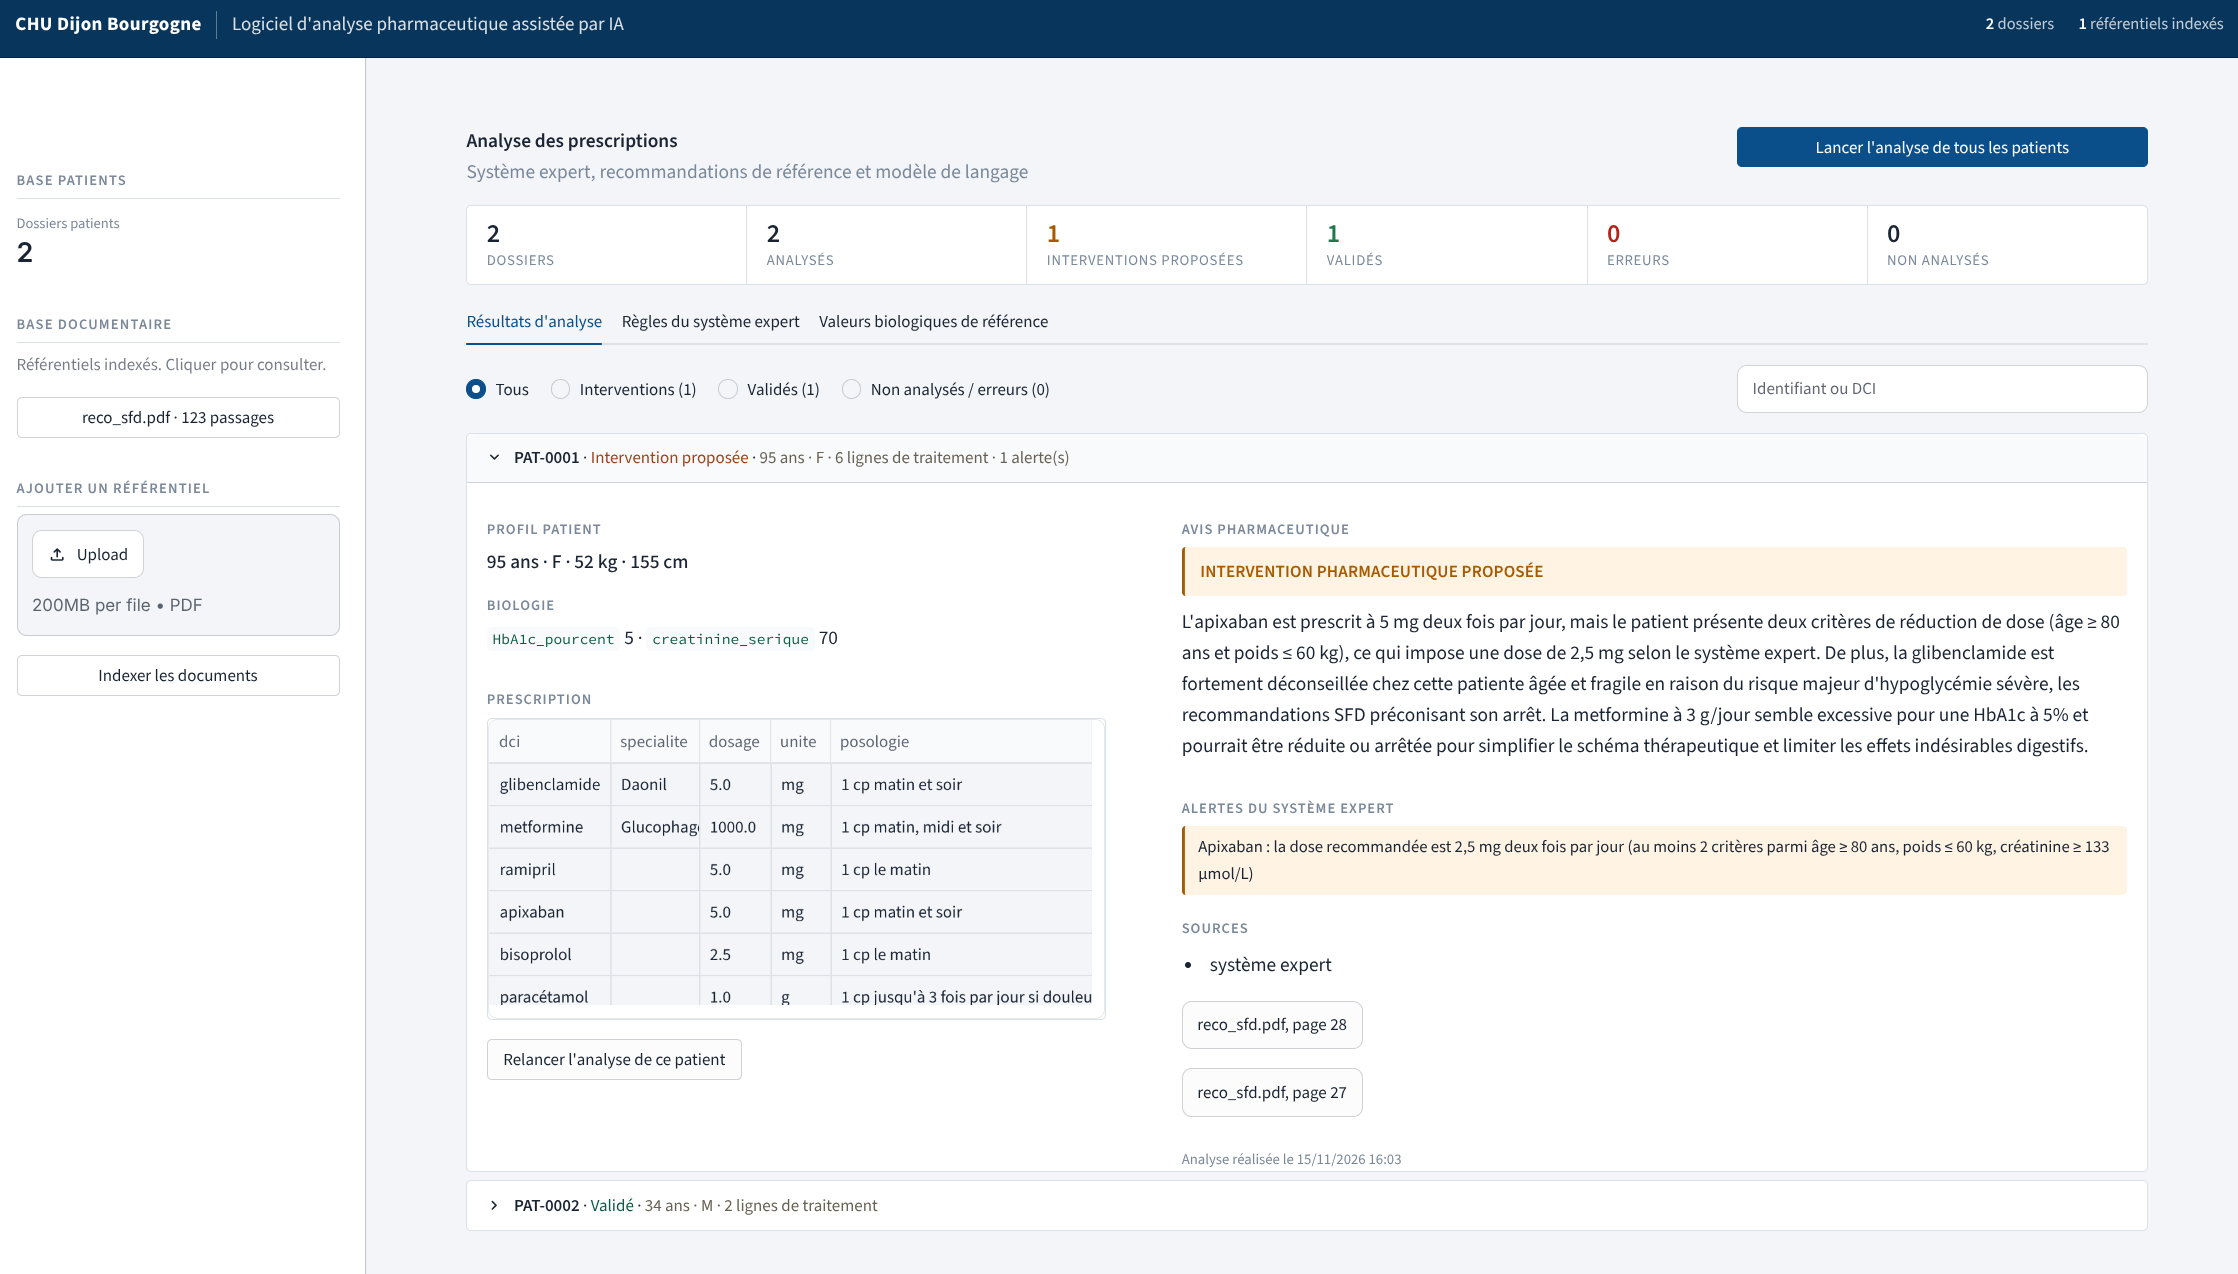
\includegraphics[width=\textwidth,height=0.9\textheight,keepaspectratio]{interface_screenshot_1.png}
\end{frame}

\begin{frame}
  \centering
  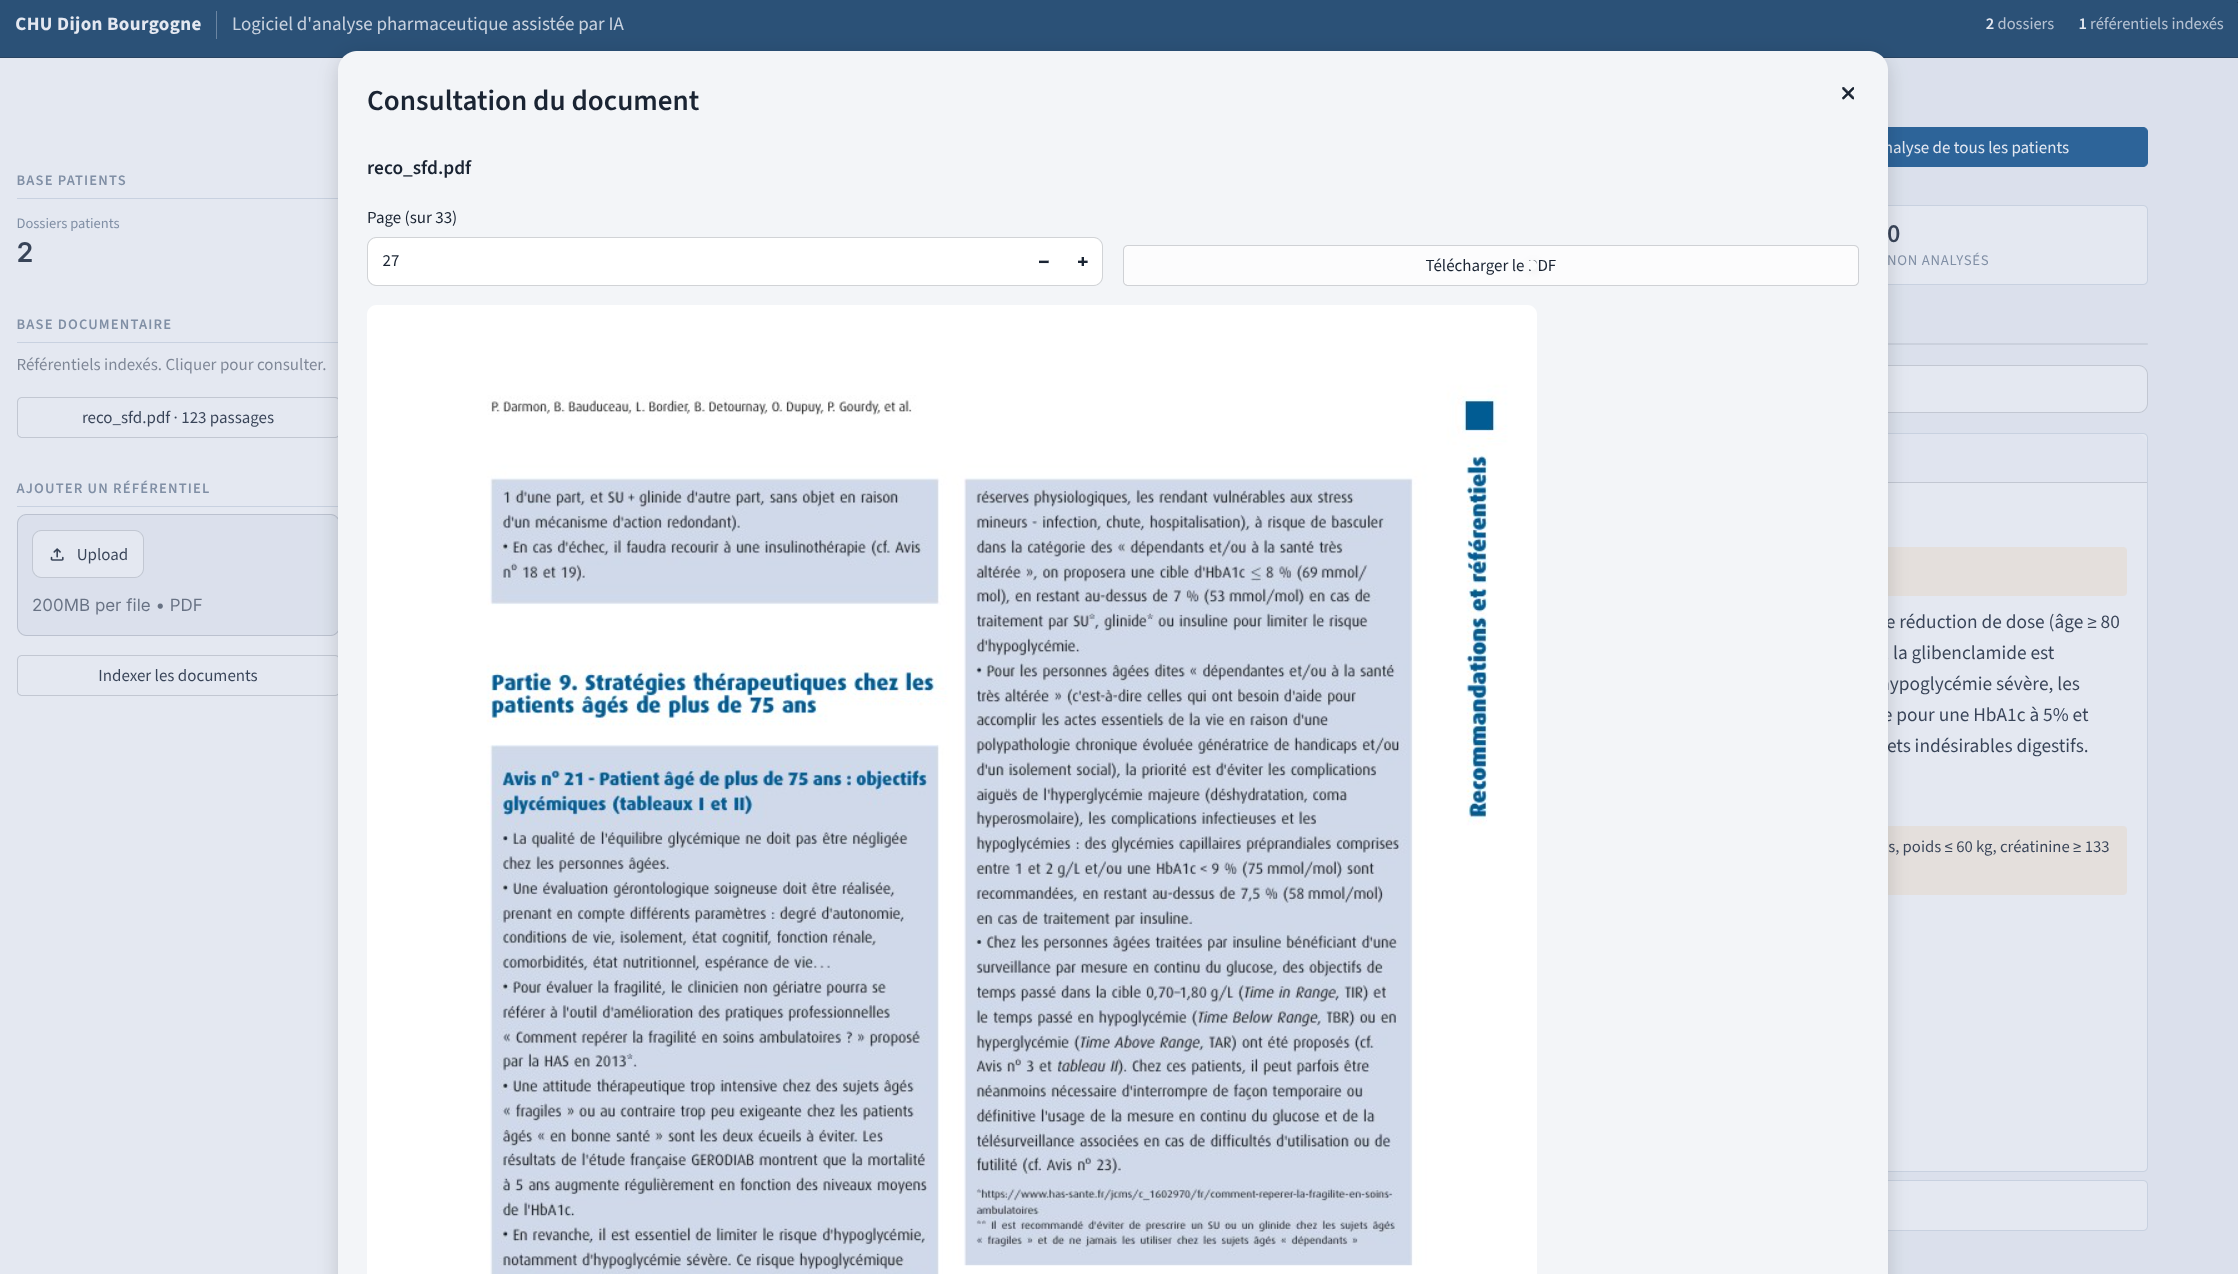
\includegraphics[width=\textwidth,height=0.9\textheight,keepaspectratio]{interface_screenshot_2.png}
\end{frame}

\begin{frame}{Liens du projet}
  \begin{itemize}
    \setlength{\itemsep}{1em}
    \item \structure{\textbf{Code source (GitHub)}} \\ {\small \url{https://github.com/naikenisen/projet_pui}}
    \item \structure{\textbf{Démonstration en ligne (Streamlit)}} \\ {\small \url{https://projetpui.streamlit.app/}}
    \item \structure{\textbf{Manuscrit de l'article (Overleaf)}} \\ {\small \url{https://www.overleaf.com/project/6afa1a238e5e3d2a0436ffc8}}
  \end{itemize}
\end{frame}



\end{document}
